
%% document format
\documentclass[12pt]{beamer}
\usetheme{default}
\usefonttheme{structurebold}


%% custom colors
\definecolor{dark}{rgb}{0.0,0.0,0.0}
\definecolor{gold}{rgb}{0.812,0.722,0.486}

%% title fonts etc
\usecolortheme[named=dark]{structure}
\setbeamerfont{footnote}{size=\tiny}


%% citation styles
%\usepackage[style=authoryear,backend=bibtex]{biblatex}
%\addbibresource{ref.bib}

%% small caption font
\usepackage{caption}
\captionsetup{font=scriptsize,labelfont=scriptsize}

%% underbraces and boxes
\usepackage{amsmath}
\usepackage{empheq}
\usepackage{bm}

%% to embed movies
\usepackage{animate}
\usepackage{hyperref}

%\usepackage{emoji}



%%%%%%%%%%%%%%%%%%%%%%%%%%%%%%%%%%%%%%%%%%%%%%%%%%%%%%%%%%%%%%
%% front matter

\title{Cubic on the Streets, Tetragonal in the Sheets: the Nature of Local Dynamic Order in CH$_3$NH$_3$PbI$_3$}
\author{Tyler C. Sterling}
\date{}
\titlegraphic{\vspace{-1cm}\includegraphics[scale=0.1]{figs/cu_logo_2.png}}


\begin{document}

%% cover slides
{
\setbeamercolor{background canvas}{bg=gold}

% --------------------------------------------------------------

\begin{frame}
\vspace{-1cm}
\titlepage
\end{frame}

% --------------------------------------------------------------

\begin{frame} %{Acknowledgements}

%\begin{block}{This project was made possible with significant contributions from collaborators at ...} 
%\end{block}

\begin{block}{collaborators at University of Colorado Boulder:}
{\color{blue}Nick Weadock (project leader) \\
Mike Toney (PI) \\
Dmitry Reznik (PI and my advisor)}
\end{block}

\vspace{1cm}
\begin{block}{and elsewhere:}
\textcolor{purple}{Ballal Ahammed \& Elif Ertekin (MD simulations)} \\
Julian A Vigil, Aryeh Gold-Parker, Ian C Smith, Matthew Krogstad, Feng Ye, David Voneshen, Peter M Gehring, Hans-Georg Steinrück, Hemamala Karunadasa
\end{block}
\end{frame}

% --------------------------------------------------------------

\begin{frame} %{Acknowledgements ...}

%\vspace{-0.5cm}
\begin{figure}
    \includegraphics[scale=0.2]{figs/doe_logo.png}
\end{figure}

\vspace{-0.5cm}
\centering
Work at CU used funding from DOE, Office of Science, Neutron Scattering Progrm

\vspace{0.5cm}
\begin{block}{Experiments done on ...}
CORELLI at the SNS (Oak Ridge) \\
Beamline 6-ID-D at the APS (Argonne) \\
MERLIN at ISIS (Rutherford Appleton)
\end{block}
\end{frame}

}

% --------------------------------------------------------------

\begin{frame} %{(nominal) structure of CH$_3$NH$_3$PbI$_3$ (MAPI)}

\textbf{(nominal) structure of CH$_3$NH$_3$PbI$_3$ (MAPI)}

\vspace{0.5cm}
\begin{figure}
    \includegraphics[width=1.0\linewidth]{figs/struct.png}
\end{figure}
\end{frame}

% --------------------------------------------------------------

\begin{frame} %{Introduction}

\textbf{Structure-function relationship in MAPI, MAPB still not known}\textcolor{red}{ ... structure still not known}

\vspace{1cm}
\begin{figure}
    \includegraphics[width=1.0\linewidth]{figs/bragg.png}
\end{figure}

\end{frame}

% --------------------------------------------------------------

\begin{frame} %{Probing the local structure}

%\vspace{-0.5cm}
\begin{figure}
    \includegraphics[width=1.0\linewidth]{figs/zb.png}
\end{figure}

\vspace{0.5cm}
Diffuse scattering shows non-trivial structure \textcolor{red}{... what is it?!} 

\end{frame}

% --------------------------------------------------------------

\begin{frame} %{Simulating MAPI}

\begin{columns}
\begin{column}{0.5\textwidth}
    Classical molecular dynamics (MD) can be used to simulate \textcolor{purple}{microscopic dynamics} \\
    ~ \\
    e.g. spectral energy density in MAPI 
\end{column}
\begin{column}{0.5\textwidth}  
    \begin{figure}
        \includegraphics[width=1.0\linewidth]{figs/elif.png}
        \caption{from \emph{Zhu, Taishan, and Elif Ertekin. Energy \&
        Environmental Science 12.1 (2019): 216-229.}}
    \end{figure}
\end{column}
\end{columns}

\end{frame}

% --------------------------------------------------------------

\begin{frame} %{Simulating scattering}

Standard expression:
\begin{equation*}
\begin{gathered}
    S(\bm{Q},\omega) = \int \langle \hat{\rho}(\bm{r},t) \hat{\rho} (0,0) \rangle \exp(i\bm{Q}\cdot \bm{r} -i \omega t) d\bm{r} dt
\end{gathered}
\end{equation*}
Time development of $\hat{\rho}$ is \textcolor{red}{many-body problem} %\emoji{skull-and-crossbones}

\vspace{1cm}
Approximate $\hat{\rho} \rightarrow \rho$ as classical
\begin{equation*}
\begin{gathered}
    S(\bm{Q},\omega) = \Big| \sum_i \underbrace{f_i(Q)}_\text{``form-factors"} \int \exp(i\bm{Q}\cdot \underbrace{\bm{r}_i(t)}_\text{trajectories} -i \omega t) dt \Big|^2
\end{gathered}
\end{equation*}
$\bm{r}_i(t)$ are straightforwardly calculated by \textcolor{blue}{classical MD} %\emoji{cowboy-hat-face}

\end{frame}

% --------------------------------------------------------------

\begin{frame}{MD vs. experiment}

\begin{figure}
    \includegraphics[width=1.0\linewidth]{figs/acns_md_vs_exp.png}
\end{figure}

\end{frame}

% --------------------------------------------------------------

\begin{frame}{Probing the local order}

\begin{figure}
    \includegraphics[scale=0.275]{figs/xds.png}
%    \includegraphics[width=1.0\linewidth]{figs/xds.png}
\end{figure}

\end{frame}

% --------------------------------------------------------------

\begin{frame}{The local order}

\begin{figure}
    \includegraphics[width=1.0\linewidth]{figs/local_order.png}
\end{figure}

\end{frame}

% --------------------------------------------------------------

\begin{frame}{2D nature of local order}

\begin{figure}
    \includegraphics[width=1.0\linewidth]{figs/local_order_2.png}
\end{figure}

\end{frame}

% --------------------------------------------------------------

\begin{frame} %{The PbI$_6$ sub-lattice}

\begin{figure}
    \includegraphics[width=0.65\linewidth]{figs/pancakes.png}
\end{figure}

Octahedra form \textcolor{purple}{2D ``pancakes"} of tetragonal-like domains

\end{frame}

% --------------------------------------------------------------

\begin{frame}{Dynamics of pancakes}
\centering
\animategraphics[autoplay,loop,scale=0.35]{20}{figs/rot_pngs/oct-}{0}{100}
\end{frame}

% --------------------------------------------------------------

{
\setbeamercolor{background canvas}{bg=gold}

\begin{frame} %{Summary}

\begin{columns}
\begin{column}{0.5\textwidth}

\textbf{Non-trivial order in PbI$_6$ sub-lattice:} \textcolor{purple}{rods in reciprocal space signal 2D ordering}

\begin{figure}
    \includegraphics[width=0.9\linewidth]{figs/rods.png}
\end{figure}

\end{column}
\begin{column}{0.5\textwidth}

\begin{figure}
    \includegraphics[width=0.9\linewidth]{figs/pancakes_2.png}
\end{figure}

\textbf{MD simulations reveal the nature of order:} \textcolor{purple}{PbI$_6$ form ``pancakes" of fluctuating tetragonal-like 2D domains}

\end{column}
\end{columns}

\end{frame}

}

% --------------------------------------------------------------

\begin{frame} %{Other sub-lattice contributions}

Total scattering:
\begin{align*}
\begin{gathered}
    S(\bm{Q},\omega) = \Big| \sum_i f_i(Q) \int \exp(i\bm{Q}\cdot \bm{r}_i(t) -i \omega t ) dt \Big|^2
\end{gathered}    
\end{align*}

Sub-lattice contributions:
\begin{align*}
\begin{gathered}
    \rho_\alpha(\bm{Q},\omega) \equiv \sum_{i \in \{ \alpha \} } f_i(Q) \exp(i\bm{Q}\cdot \bm{r}_i(t) - i\omega t) \\
    \alpha \equiv \textrm{PbI}_6 = \{ \textrm{Pb,~I} \} \\
    \alpha \equiv \textrm{MA} = \{ \textrm{C,~H,~N} \} 
\end{gathered}    
\end{align*}

``Interference" correlations:
\begin{align*}
\begin{gathered}
    S_\text{int.}(\bm{Q},\omega) = S(\bm{Q},\omega)-(\underbrace{|\rho_{\text{PbI}_6}|^2}_{S_{\text{PbI}_6}(\bm{Q},\omega)}+\underbrace{|\rho_\text{MA}|^2}_{S_\text{MA}(\bm{Q},\omega)})
\end{gathered}    
\end{align*}

\end{frame}

% --------------------------------------------------------------

\begin{frame}{Other sub-lattice contributions}

\begin{figure}
    \includegraphics[width=1.0\linewidth]{figs/ma.png}
\end{figure}

\end{frame}

% --------------------------------------------------------------

\end{document}


